\documentclass[conference]{IEEEtran}
%http://wp.internetsociety.org/ndss/wp-content/uploads/sites/25/2017/09/bare_NDSS.tex
\usepackage[utf8]{inputenc}
\usepackage[colorlinks = true,
            linkcolor = blue,
            urlcolor  = blue,
            citecolor = green,
            anchorcolor = blue]{hyperref}

\usepackage{graphicx}
\graphicspath{{figs/}}
\usepackage{booktabs}

\begin{document}
\title{Non-secure dynamic updates in DNS}

\author{\IEEEauthorblockN{Author1}
\IEEEauthorblockA{Institution1\\
someemail@somedomain.com}
\and
\IEEEauthorblockN{Author2}
\IEEEauthorblockA{Institution2\\
someemail@somedomain.com}
\and
\IEEEauthorblockN{Author3}
\IEEEauthorblockA{Institution3\\
someemail@somedomain.com}}

\maketitle



\begin{abstract}
The abstract goes here.
\end{abstract}

\section{Introduction}


\section{Background}


In this section, we introduce the necessary background about the dynamic updates in the domain name system and its security considerations.

\subsection{Brief History}

The basic specification of the domain name system was introduced over 30 years ago \cite{rfc1035,rfc1034}. 
Before then, host name to address mappings were maintained by the Network Information Center (NIC) in a single file called \texttt{HOSTS.TXT} and distributed by all hosts using FTP \cite{rfc952,rfc953}.
%
The DNS protocol initially supported queries of a statically configured database that was updated manually as it was not expected to change rapidly \cite{rfc1034}. 
However, with the introduction of the Dynamic Host Configuration Protocol (DHCP) \cite{rfc2131}, which allows to dynamically assign an IP address to each device on a network, the automatic reconfiguration mechanism for DNS  became also essential.

\begin{figure}[!ht]
\centering
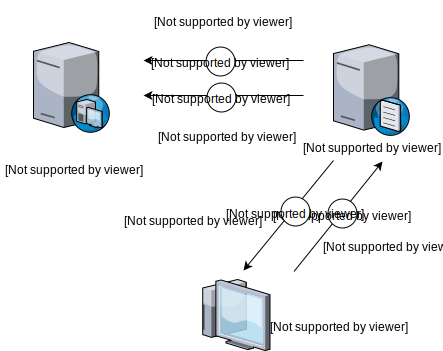
\includegraphics[width=2.5in]{figs/dhcp.pdf}
\caption{The DHCP server can be configured to register and dynamically update the host (\texttt{A}) and pointer (\texttt{PTR}) resource records with the authoritative DNS server of the zone on behalf of its DHCP-enabled clients.
%https://docs.microsoft.com/en-us/previous-versions/windows/it-pro/windows-server-2008-R2-and-2008/dd145315(v=ws.10)
}
\label{fig_dhcp}
\end{figure}

\subsection{Dynamic Updates in DNS}
%The DHCP protocol provides not only a mechanism for allocation of network addresses to Internet hosts but also can be configured to  dynamically update both the \texttt{A} and \texttt{PTR} (reverse DNS record) resource records in the DNS server on a client's behalf.

Internet services may use static IP addresses but can also dynamically change over short periods of time, on the order of hours or days \cite{gio}.
Due to the distributed nature of the domain mane system and the proliferation of its actors such as registrars or registry operators, updates to the global domain name system may take hours to propagate. 
%
\textit{Dynamic updates in DNS} is a protocol extension that addresses the problem of fast changes of DNS resource records in zone files, such as an \texttt{A} record, which provides a mapping between a domain name and an IP address.

The dynamic updates have been described in RFC 2136 \cite{rfc2136}. 
The specification supports all DNS record types.
Therefore, a client can update, add or delete any type of record, including \texttt{A}, \texttt{AAAA}, \texttt{NS}, or \texttt{TXT}.
It is often used %as an extension of
in combination with the DHCP protocol, which can be configured not only as a mechanism for allocation of network addresses to Internet hosts but also to dynamically update both \texttt{A} and \texttt{PTR} (pointer or reverse DNS) resource records in the DNS server %on a client's behalf 
on behalf of its clients (cf.~\autoref{fig_dhcp}).


%It supports all DNS record types, but often it is used only as an extension of the DHCP system, and in which the authorized DHCP servers register the client records in the DNS.


%
%Following this specification, a DNS client can add or delete any type of RR, such as A, AAAA, CNAME, or NS.

%Some servers that are maintained by certain types of Internet service providers (ISPs) are likely to change their IP address over very short periods of time, 



The proposed DNS \texttt{UPDATE} message complies with the standard DNS message format (cf. RFC 1035 \cite{rfc1035}) and is defined as follows:
\newline
\noindent
       \texttt{+----------------+}
      \newline \noindent
       \texttt{|\hspace{0.85cm} Header\hspace{0.85cm} |} contains the opcode value~(5)
      \noindent \texttt{+----------------+}
      \newline \noindent
      \texttt{|\hspace{1.16cm}Zone\hspace{1.16cm} |} specifies the zone to update
      \texttt{+----------------+}
      \newline \noindent
      \texttt{|~\hspace{0.115cm}~Prerequisite\hspace{0.115cm} |} RRs that must~(not)~preexist
      \texttt{+----------------+}
      \newline \noindent
      \texttt{|\hspace{0.95cm}Update\hspace{0.95cm} |} RRs to be added or deleted
      \texttt{+----------------+}
      \newline \noindent
      \texttt{|\hspace{0.005cm}Additional Data\hspace{-0.005cm} |} additional information (if any)
      \texttt{+----------------+}

The \texttt{Header} section contains the \texttt{UPDATE} opcode equal to~5. The \texttt{Zone} section must specify the zone name to update, i.e. a domain name (e.g.: \texttt{\url{example.com}}). The \texttt{Prerequisite} section can specify 
requirements %demanded as conditions for an update in terms of a DNS zone file content 
that must be satisfied by the DNS zone file such as existence or nonexistence of a specific resource record (RR). %, before being allowed to proceed with an update
The \texttt{Update} section contains resource record(s) to be added to or deleted from the DNS zone (e.g.:  \texttt{\url{example.com} A 10.10.10.10}), whereas \texttt{Additional Data} section can be used to supply a server with some additional information needed to, for example,  secure DNS update~\cite{rfc2136}.

When a primary master name server that supports dynamic updates receives an update request, it verifies whether all prerequisites (if any) defined by the requestor are met and whether restrictions (if any) regarding which hosts are permitted to make updates are met.
Note that if there are no restrictions defined by the DNS authoritative name server, anyone who knows the name of the zone (e.g.: \texttt{\url{example.com}}) and the name server (e.g.: \texttt{\url{ns1.example.com}}) for that zone is capable of updating its content by sending a single UDP datagram.
It can be tested using a standard \texttt{nsupdate} command\footnote{Dynamic DNS update utility: \url{https://linux.die.net/man/8/nsupdate}}.
%
%
The RFC specification also defines a case, where the request is sent to a DNS slave server that is authoritative for a given domain name.
The update request is expected to be forwarded towards the primary DNS server that can modify the zone file.

\subsection{Security Considerations}
The method described in RFC 2136 also includes a brief discussion of the security considerations and recommends using DNS Security Extensions (DNSSEC) digital signatures covering requests to secure dynamic updates and restrict requestors to those authorized to perform them %, for example, a local DHCP server 
(cf. RFC~2137~\cite{rfc2137} %, superseded by RFC~3007~\cite{rfc3007}).
and RFC~3007~\cite{rfc3007}).
If the public key security mechanism is not implemented, an authoritative name server is expected to accept the dynamic updates only from a statically preconfigured set of IP addresses.
The address match lists should be as restrictive as possible and limited to, for example, an IP address of a DHCP server.
An alternative security mechanism based on shared secret key (TSIG: Secret Key Transaction Authentication for DNS) and message authentication code was introduced three years later in RFC 2845 \cite{rfc2845} and became the most commonly used method in popular DNS software implementations.
%
%
The pressing need for DNS dynamic updates and the delayed introduction of the robust and lightweight security measures may explain a rapid uptake of the vulnerable by design, non-secure dynamic updates.
%why the vulnerable, non-secure implementations have

%and the protocol's simplicity caused a rapid uptake of the specification.


\subsection{Implementations of Dynamic Updates}

The common implementations of the DNS software, such as the open source Linux BIND \cite{bind} or the Microsoft Server DNS support vulnerable configurations, such as accepting requests from all hosts.
Some are vulnerable by default.
To date, all versions of  the Microsoft Server DNS support either an Active Directory--integrated zone, allowing only secure updates using extended TSIG or a standard primary DNS configuration that supports \textit{only} non-secure dynamic updates.
Interesting, Microsoft is aware of the vulnerability and informs the users willing to setup a non-secure implementation that ``Allowing nonsecure dynamic updates is a significant security vulnerability because updates can be accepted from untrusted sources.''
However, it remains unclear why the vulnerable version is still supported in the latest production version of the software--over 20 years after the initial release of the RFC specification.



\section{Adversary Model}
In this section, we explore the attacks that can be carried out by the adversary. We explain our infrastructure which we used to carry out attack on our victim. Finally, we present the taxonomy of attacks with discussion on their viability, stealthiness and  implications for the domain owners.

\subsection{Infrastructure Setup}
\textbf{Adversary Configuration:} Depending on the type of attack, different configurations might be required. In our setup, we assume our adversary has an access to compromised machine with public IP address. The adversary will require Dynamic DNS update utility \texttt{nsupdate} to modify the zone of our victim. Email server with forwarding is also required for more sophisticated attacks explained latter. 

\textbf{Victim Configuration:} Our victims are operating  DNS software, with BIND software. In order for the adversary to modify the records victim servers should also be vulnerable with non-secure update of records explained in previous section. In our example victim is running domain \texttt{example.com}. 


\subsection{Taxonomy of Attacks}

In a broader sense we can divide the attacks in two main categories a) Denial of Service (DoS) attack and b) man-in-the-middle (MITM) attack. In the first type of attack the adversary will be able to temporary disrupt the service of the victim. It is much easier to execute with limited stealthiness, as victim would notice the unresponsive domain and would be able to quickly fix the configuration. On the other hand, MITM attack would requires more sophistication from the adversary while being more stealthy and difficult to detect. In this section we present details of each of the attacks with our configuration 

\subsubsection{Denial of Service (DoS) Attacks} 
The DoS attack will only cause limited disruption in the service until the victim gets notified. However, these types of attacks can result in financial losses due to domain downtime or loss of customers, which might move to competitors. The adversary can cause DoS attack using one of the following records. 

\textbf{Deletion of A record of domain/sub-domain:} The adversary can delete A record with command \texttt{update delete example.com A} using nsupdate. This would delete the domain and corresponding IP address of example.com from zone file, resulting in downtime of the traffic. 

\textbf{Deletion of MX records:} Similarly, adversary can also delete MX record which will not only disrupt email service but also hinder any abuse messages sent to victim.  

\textbf{Deletion of NS record:} Deletion of NS record will be most disruptive for the victim as all available domains including email service will be un-accessible to victim and its users till the zone file is updated with correct records. 
 % Need to check following statements...

 \textbf{Deletion of delegation:} Delegated zones can be used for variety of purposes. It can be used for management of domains and subdomains or for the backup if master zone is down,  when configured as slave. If adversary successfully deletes delegation in the zone file. It would not only cause service disruption to the  domains handled by delegated server, but would also disrupt backup. 


\subsubsection{Man-in-the-middle (MITM) Attacks}
The second type of attack that adversary can utilize is MITM attack. These attacks can be more sophisticated and harder to detect. 

\textbf{Add/Update of A record to own server:}
\begin{itemize}
\item redirect traffic for disruption
\item add a subdomain and redirect info after stealing 
\item add a subdomain to launch a phising attack 
\item add a domain with domain verfication using certs to show as legitimate site 
\end{itemize}
\textbf{Add/Update MX record:} 
\begin{itemize}
\item redirect all mail to own servers to steal important information 
\item add another mx record with subdomain to use in phishing scam 
\item add an mx record with email server configured to by pass domain verification required for SSL certificates

\end{itemize}

\textbf{Add/Update delegation:}



%\section{Threat Model}
\section{Methodology}
\subsection{Datasets descriptions}
\subsection{Ethical considerations}
\subsection{Active scans}

\section{Enumeration of vulnerable resources}

\begin{table}
  \caption{Summary of vulnerable resources \label{tab:vulnerable}}
 \centering
\begin{tabular}{l*{3}{c}}
\Xhline{2\arrayrulewidth}
\#  & \textbf{\textit{Global 1}} & \textbf{\textit{Global 2}} \\
\hline
Domains & 309,687(0.095\%) & 381,965(0.108\%) \\
NS (IP addresses) & 5738(0.166\%) & 5576(0.145\%) \\
Domain--NS IP pairs & 579,186(0.018\%) & 679,930(0.014\%) \\
\Xhline{2\arrayrulewidth}
 \end{tabular}
\end{table}


\subsection{Global campaign 1}
We performed our first global campaign between \hl{need the timeframe here} using domain set specified in Table \ref{tab:data}. We were able to confirm 309,687 vulnerable domains translating into 0.095\% of all the scanned domains and 5738 (0.166\%) unique, vulnerable NSs. In total, we discovered  579,186 (0.018\%) vulnerable Domain--NS pairs (Table \ref{tab:vulnerable}). The low percentage of vulnerable resource can be explained by the broad input set that were not actively verified before vulnerability scans (\ref{sec:dataset}). 

\subsection{Global campaign 2}
Our second global campaign (\hl{need the timeframe here}) confirmed the results obtained during the first trail. We discovered 381,965(0.108\%) vulnerable domains, 5576(0.145\%) vulnerable NSs and 679,930(0.014\%) unique Domain--NS pairs. In comparison to the first global campaign, the number of vulnerable domains was increased by more than 23\%, while the number of vulnerable servers decrease by 3\% regardles the increased input set size. 
\michal{Do we need to explain those results further?}


\subsection{Short-lived domains}
\subsection{Vulnerable subdomains}
\subsection{Propagation between primary and secondary name servers - Michał}
%\begin{table}[h!]
%\begin{center}
%\caption{Propagation results. \label{tab:propagation}}
%\begin{tabular}{| c | c | c | c | c|} 
%\hline
%\textbf{Time} & \multicolumn{2}{|c|}{\textbf{Master Injects}} & \multicolumn{2}{|c|}{\textbf{Slave Injects}} \\
%\hline
%& \textbf{Primary} & \textbf{Secondary} & \textbf{Primary} & \textbf{Secondary}\\ 
%\hline
%0h & 16911 & 23474 & 829 & 57299\\ 
%\hline 
%12h & 16334 \textcolor{green}{+83} \textcolor{red}{-660}& 23396 \textcolor{green}{+330} \textcolor{red}{-408}& 451 %\textcolor{green}{+51} \textcolor{red}{-429}& 55425 \textcolor{green}{+157} \textcolor{red}{-2031} \\ 
%\hline 
%24h & 15592 \textcolor{green}{+98} \textcolor{red}{-840} & 21760 \textcolor{green}{+116} \textcolor{red}{-1752} & %712 \textcolor{green}{+163} \textcolor{red}{-2802} & 47019 \textcolor{green}{+386} \textcolor{red}{-8792} \\ 
%\hline 
%\end{tabular}
%\end{center}
%\end{table}
%We investigated propagation of injected records between primary and secondary name servers and \textit{vice versa}. \textcolor{red}{Why we're doing it?}
%For each vulnerable domain we prepared a list of primary and secondary name servers based on actively queried \texttt{NS} and \texttt{SOA} records. 
%In the first experiment, we sent injects only to primary servers and queried primary and secondary servers 3 times within 24 hours. 
%Depending on the configuration, primary servers can push new entries to secondary servers right away or wait for secondary servers to pull the changes (secondary servers should do it at least once a day). 
%Table \ref{tab:propagation} summarizes the results.
%The attack directly affected 16,911 primary servers that immediately pushed updates to 23,474 secondary servers. 
%The attack directly affected 17,092 primary servers that pushed updates to 23,920 secondary servers within one day (23,474 of which were affected immediately). 
%It means that on average, each infected primary server poisoned additional ~1.4 secondary servers.

%In our second experiment, we targeted only secondary servers. 
%If configured correctly, secondary servers are not allowed to update zones. However, a 
%The secondary server can be configured to forward an update to its primary server, which updates the zone. 
%If misconfigured, 
%In such a scenario, the primary server can accept the update as coming from a legitimate source even if the primary server may not be directly vulnerable to injects coming from unauthorized requestors.  
%The number of poisoned secondary servers rose to 57,299. 
%\textcolor{red}{Why so many? Maybe some manual analysis will reveal some interesting examples/trends from which we can hypothesize or maybe even make general conclusions?}
%However, the number of affected primary servers got decreased significantly to only 829, suggesting that update forwarding is not enabled. 
%It corresponds to ~0.27 propagation rate. 
% \textcolor{red}{Lessons learned at the end + nice table (see Table III) with less results (maybe aggregated after 24h) and more detailed caption + more analysis of the data: maybe some manual analysis and examples that could give the intuition behind the results. For example, why we managed to infect only 23k secondary by injects to primary, while we managed to make injects to 57K secondary directly. Maybe for a given domain we have more parties that provide authoritative information? What are those secondary servers that did not get updated after poisoning the primary and possibly why?}

%We queried all the servers after additional 12h and 24h. In all cases, the total number of poisoned servers decreases slightly over time. However, apart from disappearing entries, we also observed a small number of new entries that appeared in those later scans. This is due secondary servers pulling updates from master servers (when targeting primary servers) and delayed processing of forwarded updated (when targeting secondary servers). 

\begin{figure}[!hbt]
\centering
\includegraphics[width=0.8\columnwidth]{domains_vulnerability}
\caption{Domains Vulnerability}
\label{fig:domains_vulnerability}
\end{figure}

To investigate the vulnerability of different types of servers, we repeat our tests targeting different groups of DNS servers. For each vulnerable domain we prepared a list of primary and secondary name servers based on actively queried \texttt{NS} and \texttt{SOA} records. In the first experiment, we sent injects only to primary servers and queried primary and secondary servers right away and after 24 hours. In our second experiment, we targeted the secondary servers uniquely and again queried all the servers right away and after 24 hours. 

The majority of the domains can be attacked using both their primary and secondary servers(Fig. \ref{fig:domains_vulnerability}). However, more than 24,000 domains were vulnerable when attacked using one type of servers. Surprisingly, we discovered a similar amount of domains having vulnerable primary and secondary servers. 

\begin{table}[!htbp]
\centering
\caption{Propagation}
\label{tab:propagation}
\begin{tabular}{@{}lcccc@{}}
\toprule
 & \multicolumn{2}{c}{\textbf{\begin{tabular}[c]{@{}c@{}}Master\end{tabular}}} & \multicolumn{2}{c}{\textbf{\begin{tabular}[c]{@{}c@{}}Slave\end{tabular}}} \\ %\midrule
 & \multicolumn{1}{c}{\textbf{\begin{tabular}[c]{@{}c@{}}0h\end{tabular}}} & \multicolumn{1}{c}{\textbf{\begin{tabular}[c]{@{}c@{}}24h\end{tabular}}}& \multicolumn{1}{c}{\textbf{\begin{tabular}[c]{@{}c@{}}0h\end{tabular}}} & \multicolumn{1}{c}{\textbf{\begin{tabular}[c]{@{}c@{}}24h\end{tabular}}} \\ \midrule
Domains
 & 29479 & 28242 & 29883 & 25268\\ \midrule
Servers
 & 4514 & 4498 & 6526 & 6444\\ \midrule
 Propagation
 & 1643 & 1645 & 15 & 16\\ \bottomrule
\end{tabular}
\end{table}

We then investigate the evolution of the number of affected domains and servers over time (Tab. \ref{tab:propagation}. Querying affected domains directly after sending the inject reveals a similar number of domains for both primary and secondary servers. However, after 24h, the entries injected using secondary servers disappear at a much higher rate than those injected using primary servers. The entries disappear when corresponding, unaffected primary server, propagates the correct configuration to the infected secondary server. 

We also investigate the number of servers affected using both types of injects. Targeting primary servers results in a significantly lower number of affected servers. This is because of a higher number of secondary servers for each affected domains. The number of affected servers remains stable throughout our experiment. 

Finally, we investigate if a vulnerable server is able to infect other servers with an updated configuration. When targeting primary servers, we discovered more than 1,600 secondary servers that downloaded the incorrect zone information. We discovered a significantly lower number of secondary servers pushing changes to the primary one. This is understandable, as if configured correctly, secondary servers are not allowed to update zones. In both cases, the number of affected servers increase slightly over time. 

\subsection{Fingerprinting of vulnerable name servers}


\subsection{Fingerprinting of vulnerable name servers}
\section{Descriptive statistics of vulnerable resources}
\subsection{Country overview}
\subsection{Per-AS statistics}
\subsection{Per-CERT statistics}
\subsection{Per-TLD statistics}
\subsection{Popularity of affected domains}

\section{Notifications}

While non-secure dynamic updates have been a well-known misconfiguration issue for years, DNS operators still lack of the proper incentives to act.
To incentive the action of the operators of these vulnerable resources, we conducted a series of notification experiments.

Previous studies have demonstrated that directly notifying  operators does not lead to significant remediation rates~\cite{cetin2017make}. Instead, to increase the remediation rates, we notified the national CERTs and CSIRTs responsible for the hygiene of the networks where the vulnerable DNS servers are located.
Given the high concentration of vulnerable resources in a single country, before sending out the notifications at scale, we contacted directly the Japanese CERT with whom we shared all the information related to these vulnerable resources. After contacting this CERT, we measure a considerable drop (92\%) of vulnerable domains in this country by fixing 29 of the vulnerable servers.


However, even after Japan remediated most of the domains at risk in that country, more than 5,100 servers were still vulnerable leaving more than 43,000 domains at risk being exploited.
In total we conducted 8 email notification campaigns divided into 2 different phases: \textit{Phase1} targeting CERTs and CSIRTs members of the so-called 'Trusted Introducer' community; and  \textit{Phase2} targeting national and governmental CERTs. Table~\ref{tab:notif_campaign} shows an overview of the notifications that were sent out during each phase. In total, more than 200 CERTs and CSIRTs were notified via email during the time span of 6 months. The interaction with these actors was relatively low and less than 10\% actually required additional information about the scanning process. Similarly, less than 5\% of them open an automated ticket and only in 4 occasions we were notified back when the ticket was closed.

\begin{table}[!htbp]
\centering
\caption{Summary of the notification campaigns}
\label{tab:notif_campaign}
\begin{tabular}{@{}llrrr@{}}
\toprule
 & \multicolumn{1}{c}{\textbf{\begin{tabular}[c]{@{}c@{}}Notification\\ Date\end{tabular}}} & \multicolumn{1}{c}{\textbf{\begin{tabular}[c]{@{}c@{}}\#Notified\\ Entities\end{tabular}}} & \multicolumn{1}{c}{\textbf{\begin{tabular}[c]{@{}c@{}}\#Unreachable\\ Entities\end{tabular}}} & \multicolumn{1}{c}{\textbf{\#Replies}} \\ \midrule
Pilot
 & 2017-05-01 & 1 & - & \begin{tabular}[c]{@{}r@{}} 1 manual \end{tabular}\\ \midrule
\multirow{3}{*}{Phase 1} & 2017-09-06 & 44 & 2 & \begin{tabular}[c]{@{}r@{}}7 automatic\\ 16 manual\end{tabular} \\
\multicolumn{1}{c}{} & 2017-09-28 & 35 & 2 & \begin{tabular}[c]{@{}r@{}}6 automatic\\ 13 manual\end{tabular} \\
\multicolumn{1}{c}{} & 2017-10-19 & 27 & 2 & \begin{tabular}[c]{@{}r@{}}4 automatic\\ 7 manual\end{tabular} \\ \midrule
\multirow{4}{*}{Phase 2} 
 & 2018-02-14 & 168 & 5 & \begin{tabular}[c]{@{}r@{}}14 automatic \\ 40 manual \end{tabular}\\
 & 2018-02-28 & 167 & 5 &  \begin{tabular}[c]{@{}r@{}}12 automatic \\ 24 manual \end{tabular} \\
 & 2018-03-16 & 162 & 5 & \begin{tabular}[c]{@{}r@{}}12 automatic \\ 24 manual \end{tabular}  \\
 & 2018-04-12 & 76 & 5 &  \begin{tabular}[c]{@{}r@{}}7 automatic \\ 7 manual \end{tabular} \\ \bottomrule
\end{tabular}
\end{table}

A generic overview of the impact of the notifications can be seen in Fig.~\ref{fig:ts_notif} were the number of vulnerable servers and domains at risk over time is shown.
All in all, the notifications led to a 38.99\% and 39.42\%
remediation rate of the vulnerable servers and vulnerable domains respectively. These remediation rates are significantly higher than the ones reported by previous studies and signals the need to involve CERTs and CSIRTs in the remediation of vulnerabilities.  

\begin{figure}[!hbt]
    \centering
    \includegraphics[width=\columnwidth]{figs/ts_notif.pdf}
    \caption{Number of vulnerable resources over time. Each dashed line represents a notification campaign.}
    \label{fig:ts_notif}
\end{figure}

\subsection{Notification methodology}



\subsection{Phase1: TF-CSIRTs}

\begin{table}[!htbp]
    \centering
    \caption{Summary statistics by the end of the Phase 1}
    \label{tab:my_label}
    \resizebox{\columnwidth}{!}{%
\begin{tabular}{lrr}
\toprule
 & TF-CSIRTs (N = 44) & Other CSIRTs (N = 36)\\
\midrule
\bf{Remediated Servers} & ~ & ~\\
\hline
~~ N (\%) & 328 (20.4)\% & 658 (19.17)\%\\
~~ max & 62 & 220\\
~~ median & 3.0 & 2.5\\
~~ mean (sd) & 7.45 $\pm$ 11.71 & 18.28 $\pm$ 39.10\\
\hline
\bf{Vulnerable Servers} & ~ & ~\\
\hline
~~ N (\%) & 1280 (79.6)\% & 2775 (80.83)\%\\
~~ max & 235 & 911\\
~~ median & 14.5 & 13.0\\
~~ mean (sd) & 29.09 $\pm$ 43.03 & 77.08 $\pm$ 172.45\\
\hline
\bf{Remediated Domains} & ~ & ~\\
\hline
~~ N (\%) & 737 (14.24)\% & 2173 (22.29)\%\\
~~ max & 108 & 847\\
~~ median & 4.0 & 4.5\\
~~ mean (sd) & 16.75 $\pm$ 27.41 & 60.36 $\pm$ 151.84\\
\hline
\bf{Vulnerable Domains} & ~ & ~\\
\hline
~~ N (\%) & 4439 (85.76\%) & 7574 (77.71\%)\\
~~ max & 1231 & 2384\\
~~ median & 29.5 & 34.0\\
~~ mean (sd) & 100.89 $\pm$ 195.19 & 210.39 $\pm$ 494.86\\
\bottomrule
\end{tabular}}
\end{table}


\begin{figure}[!hbt]
\centering
\includegraphics[width=.8\columnwidth]{distr_cleanup_1stcampaign.pdf}
\caption{Remediation rate of the DNS servers during the first campaign}
\end{figure}

\begin{figure}[!hbt]
\centering
\includegraphics[width=.8\columnwidth]{tfcsirt_server.pdf}
\caption{Remediation rate of the DNS servers during the first campaign}
\end{figure}

\begin{figure}[!hbt]
\centering
\includegraphics[width=.8\columnwidth]{tfcsirt_domain.pdf}
\caption{Remediation rate of the domains during the first campaign }
\end{figure}
\begin{figure}[!hbt]
\centering
\includegraphics[width=.8\columnwidth]{figs/surv_tfcsirt-types.pdf}
\caption{Server remediation rate depending of the CSIRT constituency type }
\end{figure}


\subsection{Analyzing the remediation success}
\subsection{Lessons learned}
\section{Related work}

%%%%%%%%%%%%%%%%%% DNSSEC %%%%%%%%%%%%%%%%%%%%%%%%%%%%%%%%%%%%%%%%
\subsection{DNSSEC}
\cite{goldberg2015nsec5} - The paper studes DNSSEC with NSEC and NSEC3 records, and shows that it inherently suffers from zone enumeration. They then propose a new construction that uses online public-key cryptography to solve the problem of DNSSEC zone enumeration - NSEC5

\cite{van2015making} - DNSSEC adds digital signatures to the DNS, significantly increasing the size of DNS responses. This means DNSSEC is more susceptible to packet fragmentation and makes DNSSEC an attractive vector to abuse in amplification-based denial-of-service attacks. Additionally, key management policies are often complex. This makes DNSSEC fragile and leads to operational failures. In this paper, we argue that the choice for RSA as default cryptosystem in DNS- SEC is a major factor in these three problems. We show that  elliptic curve cryptography (EC-DSA and EdDSA) are highly attractive for use in DNSSEC, although they also have disadvantages. To address these, we have initiated research that aims to investigate the viability of deploying ECC at a large scale in DNSSEC.

\cite{lian2013measuring} - We have performed a large-scale measurement of the effects of DNSSEC on client name resolution us- ing an ad network to collect results from over 500,000 geographically-distributed clients. Our findings corroborate those of previous researchers in showing that a relatively small fraction of users are protected by DNSSEC-validating resolvers. And we show, for the first time, that enabling DNSSEC measurably increases end-to-end resolution failures. For every 10 clients that are protected from DNS tampering when a domain deploys DNSSEC, approximately one ordinary client (primarily in Asia) becomes unable to access the domain.

\cite{wander2013measuring} - In this paper we present a methodology to determine whether a client is protected by DNSSEC
validation. We applied our methodology over a period of 7 months collecting results from different data sources. After data cleaning, we gathered 131,320 results from 98,179 distinct IP addresses, out of which 4.8\% had validation enabled. The ratio varies significantly per country, with Sweden, the Czech Republic and the United States having the largest ratios of validating clients in the field.

\cite{rasti2015temporal} - We introduce temporal lensing—a technique that concentrates a relatively low-bandwidth flood into a short, high-bandwidth pulse. By leveraging existing DNS infrastructure, we experimentally explore lensing and the properties of the pulses it creates. We also show how attackers can use lensing to achieve peak bandwidths more than an order of magnitude greater than their up- load bandwidth. While formidable by itself in a pulsing DoS attack, we note how lensing can be compatibly combined with amplification attacks to potentially allow attackers to produce pulses with peak bandwidths orders of magnitude larger than their own.

\cite{vissers2017exploring} - This study extensively scrutinizes 14 months of registration data to identify large-scale malicious campaigns present in the .eu TLD. We explore the ecosystem and modus operandi of elaborate cybercriminal entities that recurrently register large amounts of domains for one-shot, malicious use. Although these malicious domains are short-lived, by in- corporating registrant information, we establish that at least 80.04\% of them can be framed in to 20 larger campaigns with varying duration and intensity. We further report on insights in the operational aspects of this business and observe, amongst other findings, that their processes are only partially automated. Finally, we apply a post-factum clustering process to validate the campaign identification process and to automate the ecosystem analysis of malicious registrations in a TLD zone.

\cite{chung2017understanding} - In this paper, we investigate the underlying reasons why DNSSEC adoption has been remarkably slow. We focus on registrars, as most TLD registries already support DNSSEC and registrars often serve as DNS operators for their customers. Our study uses large-scale, longitudinal DNS measurements to study DNSSEC adoption, coupled with experiences collected by trying to deploy DNSSEC on domains we purchased from leading domain name registrars and resellers. Overall, we find that a select few registrars are responsible for the (small) DNSSEC deployment today, and that many leading registrars do not support DNSSEC at all, or require customers to take cumbersome steps to deploy DNSSEC. Further frustrating deploy- ment, many of the mechanisms for conveying DNSSEC information to registrars are error-prone or present security vulnerabilities. Finally, we find that using DNSSEC with third-party DNS operators such as Cloudflare requires the domain owner to take a number of steps that 40\% of domain owners do not complete. Having identified several operational challenges for full DNSSEC deployment, we make recommendations to improve adoption.

\cite{van2014dnssec} - We perform a detailed measurement on a large dataset of DNSSEC-signed domains, covering 70\% (2.5 million) of all signed domains in operation today, and compare the potential for amplification attacks to a representative sample of domains without DNSSEC. At first glance, the outcome of these measurements confirms that DNSSEC indeed worsens the DDoS phenomenon. Closer examination, however, gives a more nuanced picture. DNSSEC really only makes the situation worse for one particular query type (ANY), for which responses may be over 50 times larger than the original query (and in rare cases up to 179x). We also discuss a number of mitigation strategies that can have immediate impact for operators and suggest future research directions with regards to these mitigation strategies.

%%%%%%%%%%%%%%%%%% MEASUREMENTS %%%%%%%%%%%%%%%%%%%%%%%%%%%%%%%%%%%%%%%%
\subsection{Measurements}
\cite{schomp2013measuring} - The paper presents methodologies for efficiently discovering the complex client-side DNS infrastructure. It further develops measurement techniques for isolating the behavior of the distinct actors in the infrastructure. Using these strategies, we study various aspects of the client-side DNS infrastructure and its behavior with respect to caching, both in aggregate and separately for different actors.


\cite{jones2016detecting} - We present techniques for detecting unauthorized DNS root servers in the Internet using primarily endpoint-based measurements from RIPE Atlas, supplemented with BGP routing announcements from RouteViews and RIPE RIS. The first approach analyzes the latency to the root server and the second approach looks for route hijacks.

\cite{fiebig2017something} - We collect a new IPv6 addresses dataset spanning more than 5.8 million IPv6 addresses by exploiting DNS’ denial of existence semantics (NXDOMAIN). This paper documents our efforts in obtaining new datasets of allocated IPv6 addresses, so others can avoid the obstacles we encountered.

\cite{fiebig2018rdns} - We observe that the share of non-authoritatively answerable IPv4 rDNS queries reduced since earlier studies and IPv6 rDNS has less non-authoritatively answerable queries than IPv4 rDNS. Furthermore, we compare passively collected datasets with actively collected ones, and we show that they enable observing the same effects in rDNS data. While highlighting oppor- tunities for future research, we find no immediate challenges to the use of rDNS as active and passive data-source for Internet measurement research.

\cite{liang2013measuring} - We surveyed the latency of upper DNS hierarchy from 19593 vantage points around the world to investigate the impact of uneven distribution of top level DNS servers on end-user latency. Our findings included: 1) generally top level DNS servers served Internet users efficiently, with median latency 20.26ms for root, 42.64ms for .com/.net, 39.07ms for .org; 2) quality of service was uneven, Europe and North America were the best while Africa and South America were 3 to 6 times worse; 3) most of the root servers performed well in Europe and North America, but only F, J, L roots showed low query latency in other continents; 4) query latency of F and L roots showed that only about 60\% resolvers were routed to the nearest anycast instances. We also revealed two problems that lead to constantly large query latency (6s-18s) for resolvers.

\cite{jonker2016measuring} - In this paper, we investigate the adoption of cloud-based DPSs worldwide. We focus on nine leading providers. Our outlook on adoption is made on the basis of active DNS measurements. We introduce a methodology that allows us, for a given domain name, to determine if traffic diversion to a DPS is in effect. It also allows us to distinguish various methods of traffic diversion and protection. For our analysis we use a long-term, large-scale data set that covers well over 50\% of all names in the global domain namespace, in daily snapshots, over a period of 1.5 years

%%%%%%%%%%%%%%%%%% SECURITY %%%%%%%%%%%%%%%%%%%%%%%%%%%%%%%%%%%%%%%%

\subsection{Security}
\cite{kountouras2016enabling} - Internet miscreants make extensive use of short-lived disposable domains to promote a large variety of threats and support their criminal network operations. we have created a system, Thales, that actively queries and collects records for massive amounts of domain names from various seeds. These seeds are collected from multiple public sources and, therefore, free of privacy concerns. The results of this effort will be opened and made freely available to the research community. With three case studies we demonstrate the detection merit that the collected active DNS datasets contain. We show that (i) more than 75\% of the domain names in public black lists (PBLs) appear in our datasets several weeks (and some cases months) in advance, (ii) existing DNS research can be implemented using only active DNS, and (iii) malicious campaigns can be identified with the signal provided by active DNS.


\cite{dietrich2018investigating} - We investigate the operators’ perspective on security misconfigurations to approach the human component of this class of security issues. We focus our analysis on system operators, as although they are the relevant actors managing the affected sys- tems, they have not yet received significant attention by prior research. We follow an inductive approach and apply a multi-step empirical methodology: (i) a qualitative study to understand how to approach the target group and measure the misconfiguration phenomenon, and (ii) a quantitative survey rooted in the qualitative data. We then provide the first analysis of system operators’ perspective on security misconfigurations, and we determine the factors that operators perceive as the root causes. Based on our findings, we provide practical recommendations on how to reduce security misconfigurations’ frequency and impact.


\cite{borgolte2018cloud} - we discover a substantial number of stale DNS records that point to available IP addresses in clouds, yet, are still actively attempted to be accessed. Often, these records belong to discontinued services that were previously hosted in the cloud. We demonstrate that it is practical, and time and cost efficient for attackers to allocate IP addresses to which stale DNS records point. An attacker can impersonate the service using a valid certificate trusted by all major operating systems and browsers. The attacker can then also exploit residual trust in the domain name for phishing, receiving and sending emails, or possibly distribute code to clients that load remote code from the domain (e.g., loading of native code by mobile apps, or JavaScript libraries by websites). An aggressive attacker could execute the attack in less than 70 seconds, well below common time-to-live (TTL) for DNS records. In turn, it means an attacker could exploit normal service migrations in the cloud to obtain a valid SSL certificate for domains owned and managed by others, and, worse, that she might not actually be bound by DNS records being (temporarily) stale, but that she can exploit caching instead.

\cite{lever2016domain} - Any individual that re-registers an expired domain implicitly inherits the residual trust associated with the domain’s prior use. We find that adversaries can, and do, use malicious re-registration to exploit domain ownership changes—undermining the security of both users and systems. In fact, we find that many seemingly disparate security problems share a root cause in residual domain trust abuse. With this study we shed light on the seemingly unnoticed problem of residual domain trust by measuring the scope and growth of this abuse over the past six years. To help address this problem, we propose a technical remedy and discuss several policy remedies. For the former, we develop Alembic, a lightweight algorithm that uses only passive observations from the Domain Name System (DNS) to flag potential domain ownership changes. We identify several instances of residual trust abuse using this algorithm, including an expired APT domain that could be used to revive existing infections.

\cite{kuhrer2015going} - Since several years, millions of recursive DNS resolvers are-deliberately or not—open to the public. This, however, is counter intuitive, since the operation of such openly accessible DNS resolvers is necessary in rare cases only. Furthermore, open resolvers enable both amplification DDoS and cache snooping attacks, and can be abused by attackers in multiple other ways. We thus find open recursive DNS resolvers to remain one critical phenomenon on the Internet. In this paper, we illuminate this phenomenon by analyzing it from two different angles. On the one hand, we study the landscape of DNS resolvers based on empirical data we collected for over a year. We analyze the changes over time and classify the resolvers according to device type and software version. On the other hand, we take the viewpoint of a client and measure the response authenticity of these resolvers. Besides legitimate redirections (e.g., to captive portals or router login pages), we find millions of resolvers to deliberately manipulate DNS resolutions (i.e., return bogus IP address information). To understand this threat in more detail, we systematically analyze non-legitimate DNS responses and reveal open DNS resolvers that manipulate DNS resolutions to censor communication channels, inject advertisements, serve malicious files, perform phishing, or redirect to other kinds of suspicious or malicious activities.

\cite{moura2016anycast} - This paper provides the first evaluation of several IP anycast services under stress with public data. Our subject is the Internet’s Root Domain Name Service, made up of 13 independently designed services (“letters”, 11 with IP anycast) run- ning at more than 500 sites. Many of these services were stressed by sustained traffic at 100x normal load on Nov. 30 and Dec. 1, 2015. We use public data for most of our analysis to examine how different services respond to stress, and identify two policies: sites may absorb attack traffic, containing the damage but reducing service to some users, or they may withdraw routes to shift both good and bad traffic to other sites. We study how these deployment policies resulted in different levels of service to different users during the events. We also show evidence of collateral damage on other services located near the attacks.

\cite{lever2013core} - Using DNS traffic collected over the course of three months from a major US cellular provider as well as a major US non- cellular Internet service provider, we identify the DNS domains looked up by mobile applications, and analyze information related to the Internet hosts pointed to by these domains. We make several important observations. The mobile malware found by the research community thus far appears in a minuscule number of devices in the network: 3,492 out of over 380 million (less than 0.0009\%) observed during the course of our analysis. This result lends credence to the argument that, while not perfect, mobile application markets are currently providing adequate security for the majority of mobile device users. Second, we find that users of iOS devices are virtually identically as likely to communicate with known low reputation domains as the owners of other mobile platforms, calling into question the conventional wisdom of one platform demonstrably providing greater security than another. Finally, we observe two malware campaigns from the upper levels of the DNS hierarchy and analyze the lifetimes and network properties of these threats. We also note that one of these campaigns ceases to operate long before the malware associated with it is discovered suggesting that network-based countermeasures may be useful in the identification and mitigation of future threats.

\cite{pereira2018dictionary} - In this paper, we design and implement a method called WordGraph for extracting dictionaries used by the Domain Generation Algorithms (DGAs) based solely on DNS traffic. Our result immediately gives us an efficient mechanism for detecting this elusive, new type of DGA, without any need for reverse engineering to extract dictionaries. Our experimental results on data from known Dictionary-AGDs show that our method can extract dictionary information that is embedded in the malware code even when the number of DGA domains is much smaller than that of legitimate domains, or when multiple dictionaries are present in the data. This allows our approach to detect Dictionary-AGDs in real traffic more accurately than state-of-the-art methods based on human defined features or featureless deep learning approaches.


\section{Conclusions}

\bibliographystyle{IEEEtranS}
%TODO: add file for biblio
\bibliography{imcbib,biblio} 

\end{document}
